\section{pliki obiektowe}
\subsection{format plików obiektowych}
\begin{frame}[t]\frametitle{Nagłówki ELF}
  \begin{figure}
    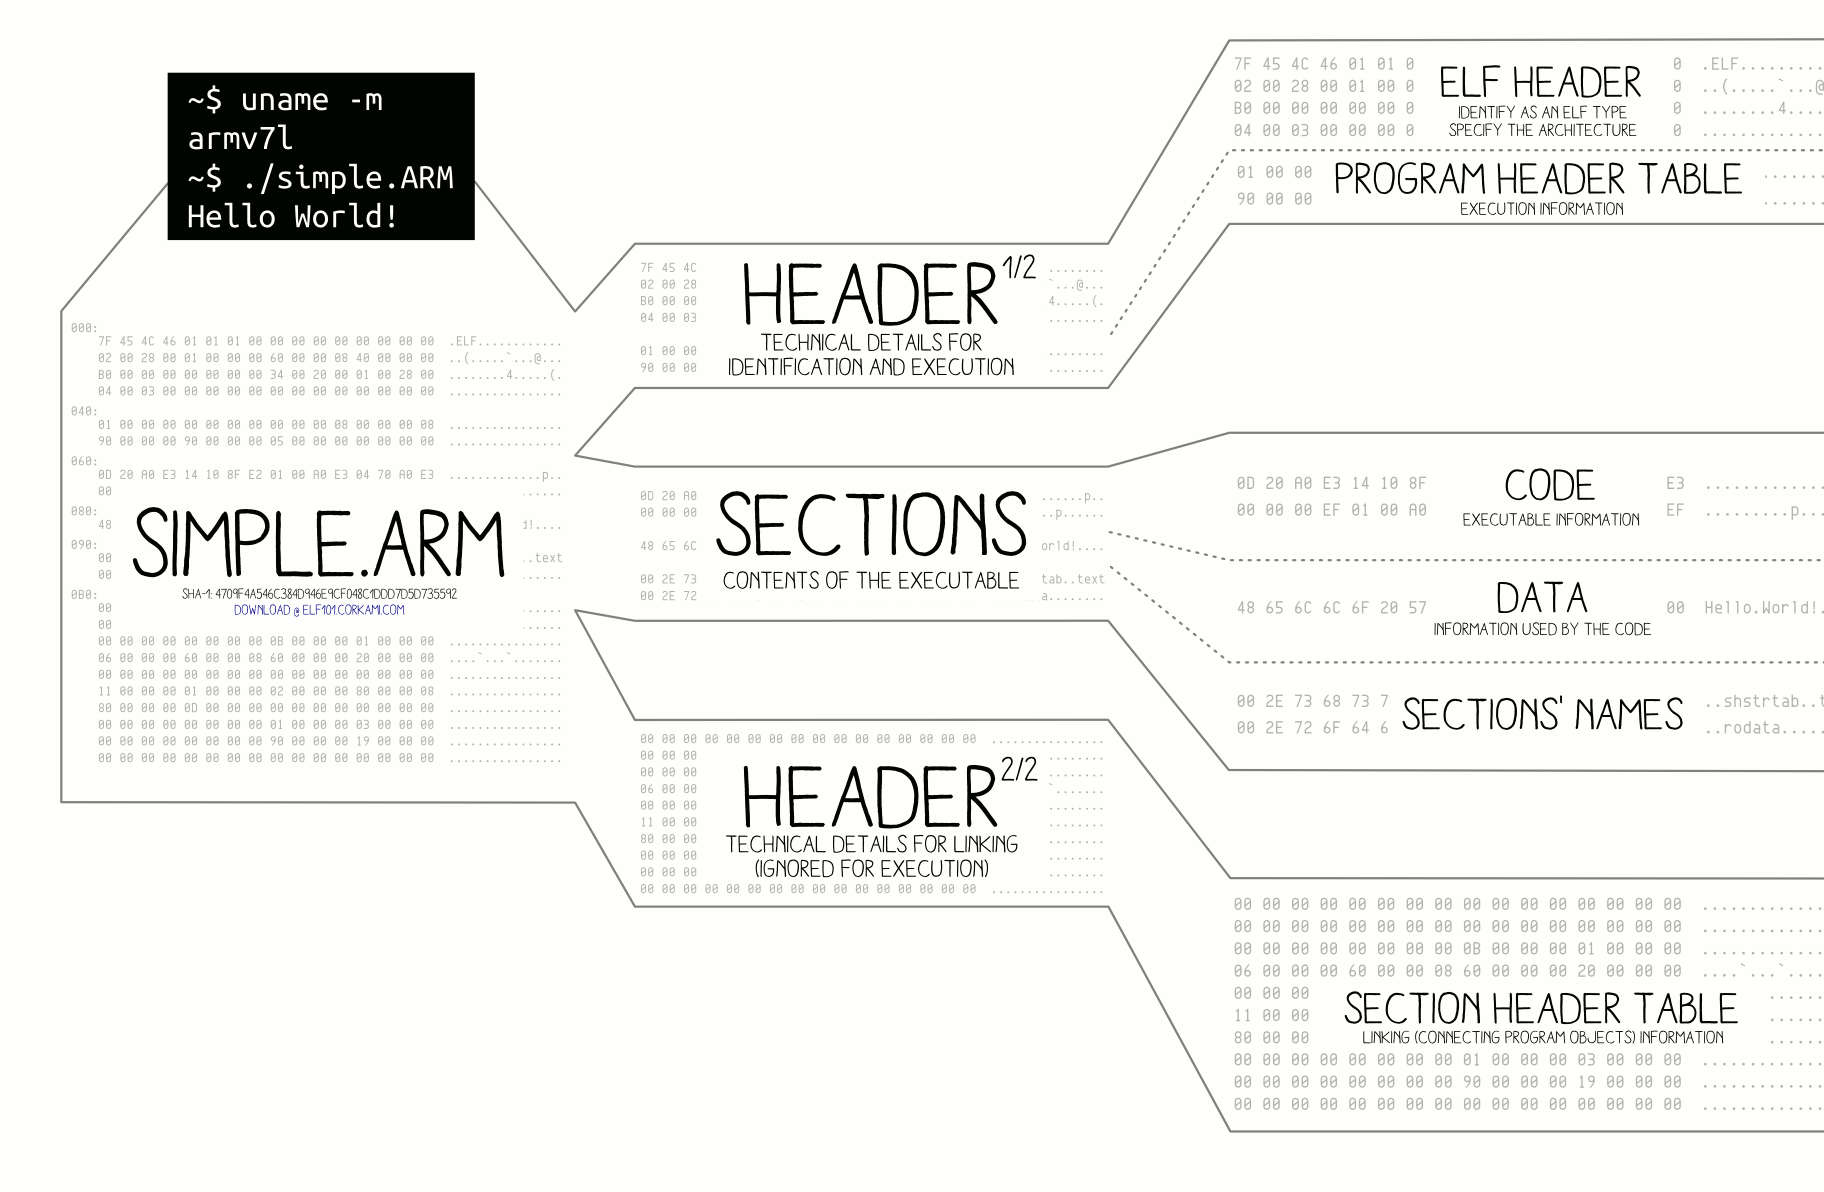
\includegraphics[width=0.9\textwidth]{ELFHeader.png}
    \caption{budowa pliku ELF \cite{ELFHeader}}
  \end{figure}
\end{frame}

\begin{frame}[t]\frametitle{ELF}
  \cite{ELF}Najważniejsze sekcje zawierają:
  \begin{itemize}
  \item{.bss --- } niezainicjowane zmienne, sekcja \textbf{.bss} zajmuje
    nieznaczne ilości pamięci, ponieważ zawiera jedynie informacje o
    zmiennych, a nie przechowuje ich wartości
  \item{.text --- } wykonywalne części programu
  \item{.data --- } zainicjowane wartości
  \end{itemize}
\end{frame}

\begin{frame}[t]\frametitle{Sekcja vs Segment}

  \textbf{Sekcje} występują przed procesem linkowania i dzielimy je na:
  \begin{itemize}
  \item ``raw data'' -- np. .text, .data itd ...
  \item ``metadata'' -- np. .symtab, .strtab itd ...
  \end{itemize}

  sekcje zawierające metadane nie są konieczne do uruchomienia programu,
  ale stanową źródło informacji dla debugerów, i programów analizujących
  pliki binarne
  [\url{przyklady/strip}]
  
  \textbf{Segmenty} występują po procesie linkowania i zawierają informacje jak
  system operacyjny ma je załadować do pamięci
\end{frame}

\begin{frame}[t]
  \begin{figure}
    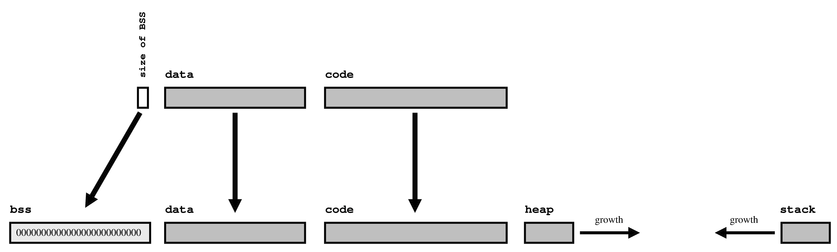
\includegraphics[width=0.9\textwidth]{loading.png}
    \caption{Proces ładowania programu do pamięci\cite{lurklurk}}
  \end{figure}

\end{frame}

\subsection{Rodzaje plików obiektowych}
\begin{frame}
  \begin{itemize}
  \item Pliki przesuwalne (Relocatable)
  \item Pliki wykonywalne (Executable)
  \item Pliki współdzielone (Shared Objects)
  \end{itemize}
\end{frame}
\begin{frame}[t]\frametitle{Przesuwalne (relocatable) pliki obiektowe}
  \begin{alertblock}{}
    Przesuwalne pliki obiektowe to takie których funkcje i zmienne nie są
    przywiązane do adresu, ale do symboli. \cite{Carson}
  \end{alertblock}


  Plik źródłowy:
  
  \lstinputlisting[language=C++, frame=single,
  firstline=2]{przyklady/00_relocatable/00.c}

  [\url{przyklady/00_relocatable}]

\end{frame}

\subsubsection{Klasy symboli ( nm )}

\begin{frame}[t]\frametitle{Wybrane klasy symboli w pliku obiektowym \cite{nmMan} }
  \begin{itemize}
  \item B - symbol jest w sekcji BSS ( niezainicjowany)
  \item C - Wspólny symbol, nie zainicjowane
  \item D - zainicjowane symbol
  \item R - tylko do odczytu
  \item T - symbol jest w sekcji text (code)
  \item U - symbol niezdefiniowany
  \end{itemize}
  
\end{frame}

\begin{frame}

  Przykład użycia programu nm na pliku obiektowym:
  \begin{table}[h]
    \begin{tabular}{lll}
      Wartość & Klasa & Nazwa\\
      0000000000000000&D&global\_initialized\_variable\\
      0000000000000004&C&global\_variable\\
      0000000000000013&t&local\_function\\
      0000000000000021&T&main\\
      0000000000000000&T&not\_implemented\_function\\
    \end{tabular}
  \end{table}
  
\end{frame}


\begin{frame}[t]\frametitle{Wykonywalne (executable) pliki obiektowe}
  \lstinputlisting[language=C++, frame=single,
  firstline=1]{przyklady/01_executable/01.c}
  [\url{przyklady/01_executable}]

  binarny plik wykonywalny zawiera adresy, natomiast przenośny plik obiektowy
  wszystkie adresy ma ustawione na 0

\end{frame}

